% https://tex.stackexchange.com/a/758843

\documentclass[tikz,border=5pt]{standalone}

\begin{document}
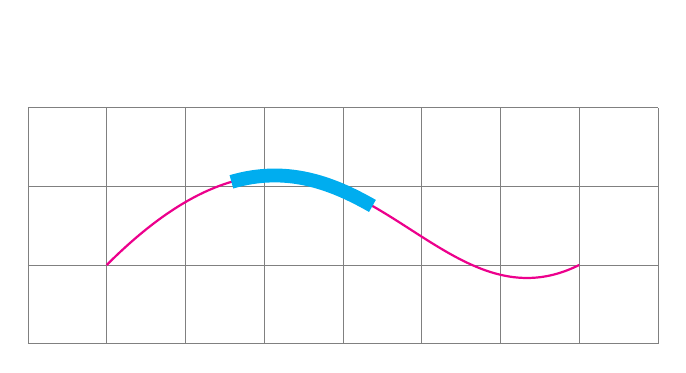
\begin{tikzpicture}
  \draw[help lines] (-1,-1) grid (7,2);

  \coordinate (P0) at (0,0);
  \coordinate (P1) at (3,3);
  \coordinate (P2) at (4,-1);
  \coordinate (P3) at (6,0);

  \draw[thick,magenta] (P0) .. controls (P1) and (P2) .. (P3);

  \draw[line width=5pt,cyan]
    \pgfextra{
      \pgfpathcurvebetweentime{0.2}{0.5}
        {\pgfpointanchor{P0}{center}}
        {\pgfpointanchor{P1}{center}}
        {\pgfpointanchor{P2}{center}}
        {\pgfpointanchor{P3}{center}}
    };
\end{tikzpicture}
\end{document}
